\section{Розгортання програмного продукту}
\subsection{Інструкція з встановлення}
\begin{sloppy}
\begin{enumerate}
\item Встановити та налаштувати web-сервер Apache, інтерпретатор PHP5 не нижче версії 5.4, СКБД MySQL 5 або MariaDB 5. Для запуску сервера та клієнта на одній машині можна скористатися XAMPP з \url{https://www.apachefriends.org/ru/index.html}.
\item Скачати та розпакувати архів: \url{https://github.com/bodqhrohro/knp2014/archive/master.zip}.
\item Розпакувати вміст каталогу src з архіву до каталогу сторінок сайту. за необхідності налаштувати домен.
\item Встановити PHPMyAdmin (\url{https://www.phpmyadmin.net/}), перейти на вкладку "Імпорт" та вибрати файл deploy.sql з каталогу src. Впевнитися, що операція імпорту пройшла успішно.
\item Відкрити у текстовому редакторі файл config.php з кореневого каталогу сайту та вказати там IP чи домен СКБД, логін та пароль для доступу до БД, а також домен, на якому розміщено сайт. Зберегти файл.
\item Відкрити домен, на якому розміщено сайт, у браузері. Впевнитися, що відображається форма входу.\\
\includegraphics[width=17cm]{scrns/login.png}\imglabel{Форма входу}
\end{enumerate}
\end{sloppy}
\subsection{Інструкція з використання}
Демонстраційну копію системи розміщено на \url{http://php-bodqhrohro.rhcloud.com/knp2014/}.

В щойно встановленій системі є чотири тестових користувачі: адміністратор asdf, оператор fdsa, переглядачі pnd та qwer. Паролі для них, відповідно: adsf, fdsa, pnd, qwer. Можна запрошувати створення нових користувачів. Натисніть кнопку "Реєстрація" у верхньому правому кутку. введіть логін нового користувача та пароль. Підтвердіть форму, перейдіть знов на сторінку входу та спробуйте увійти під користувачем asdf. Відкриється головний інтерфейс системи --- стрічка меню.
\\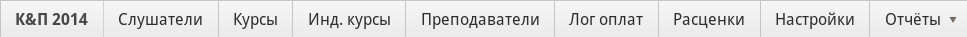
\includegraphics[width=17cm]{scrns/menu.png}\imglabel{Головне меню}

При реєстрації нового користувача адміністратори отримують сповіщення. Відкрийте з головного меню панель сповіщень та ввімкніть режим "Детально".
\begin{center}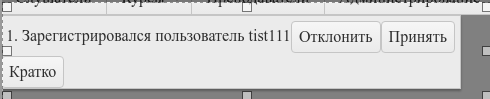
\includegraphics[width=10cm]{scrns/notifications.png}\end{center}\imglabel{Сповіщення}

Можна підтвердити користувача, після чого під ним можна буде зайти, або видалити його. Таким же чином оброблюються заявки слухачів на запис на курси. Щоб сховати панель, натисніть пункт "Сповіщення" ще раз.

Пункт "Вихід" головного меню викликає завершення сесії користувача та перехід на екран входу. Підменю "Звіти" містить пункти, що відкривають форми налаштування звітів. Решта пунктів відкривають таблиці. Натисніть, приміром, пункт "Слухачі". Відкриється таблиця для роботи зі слухачами.

Можна додавати нові рядки за допомогою кнопки на панелі інструментів, видаляти їх за допомогою кнопки зправа та редагувати, клацнувши на потрібній комірці. Змінені комірки підсвічуються. Всі зміни в таблиці не синхронізуються із сервером автоматично --- для цього слугує кнопка "Зберегти зміни". Якщо вміст якоїсь комірки перешкоджає збереженню, вона залишиться підсвіченою.

Таблиці "Слухачі" та "Курси" мають у кожному рядку підтаблиці, що дозволяють записувати слухачів на курси та працювати з оплатами. Розгортаються підтаблиці клацанням по трикутнику з лівого краю рядка. У підтаблицях не можна безпосередньо редагувати комірки, оплата вводиться у формі, що викликається кнопкою "Змінити". При поверненні грошей слухачеві вводиться від'ємна оплата. Додаються слухачі або групи з випадаючого списку; для слухачів він представлений у вигляді дерева з прапорцями, що дозволяє зручно додавати на курс цілі університетські групи та шукати слухачів за групами замість довгого алфавітного списку чи форми пошуку. Слухачі не з університету або з невідомої групи відображаються у піддереві "Інші".

Коли треба згенерувати звіт, виберіть потрібний звіт з випадаючого меню. За необхідності введіть діапазон дат та натисніть кнопку "Створити звіт". Якщо звіт не відкривається у браузері, його можна зберегти та відкрити будь-яким переглядачем PDF та з нього ж відправити на друк.
